\documentclass{article}\usepackage[]{graphicx}\usepackage[]{xcolor}
% maxwidth is the original width if it is less than linewidth
% otherwise use linewidth (to make sure the graphics do not exceed the margin)
\makeatletter
\def\maxwidth{ %
  \ifdim\Gin@nat@width>\linewidth
    \linewidth
  \else
    \Gin@nat@width
  \fi
}
\makeatother

\definecolor{fgcolor}{rgb}{0.345, 0.345, 0.345}
\newcommand{\hlnum}[1]{\textcolor[rgb]{0.686,0.059,0.569}{#1}}%
\newcommand{\hlsng}[1]{\textcolor[rgb]{0.192,0.494,0.8}{#1}}%
\newcommand{\hlcom}[1]{\textcolor[rgb]{0.678,0.584,0.686}{\textit{#1}}}%
\newcommand{\hlopt}[1]{\textcolor[rgb]{0,0,0}{#1}}%
\newcommand{\hldef}[1]{\textcolor[rgb]{0.345,0.345,0.345}{#1}}%
\newcommand{\hlkwa}[1]{\textcolor[rgb]{0.161,0.373,0.58}{\textbf{#1}}}%
\newcommand{\hlkwb}[1]{\textcolor[rgb]{0.69,0.353,0.396}{#1}}%
\newcommand{\hlkwc}[1]{\textcolor[rgb]{0.333,0.667,0.333}{#1}}%
\newcommand{\hlkwd}[1]{\textcolor[rgb]{0.737,0.353,0.396}{\textbf{#1}}}%
\let\hlipl\hlkwb

\usepackage{framed}
\makeatletter
\newenvironment{kframe}{%
 \def\at@end@of@kframe{}%
 \ifinner\ifhmode%
  \def\at@end@of@kframe{\end{minipage}}%
  \begin{minipage}{\columnwidth}%
 \fi\fi%
 \def\FrameCommand##1{\hskip\@totalleftmargin \hskip-\fboxsep
 \colorbox{shadecolor}{##1}\hskip-\fboxsep
     % There is no \\@totalrightmargin, so:
     \hskip-\linewidth \hskip-\@totalleftmargin \hskip\columnwidth}%
 \MakeFramed {\advance\hsize-\width
   \@totalleftmargin\z@ \linewidth\hsize
   \@setminipage}}%
 {\par\unskip\endMakeFramed%
 \at@end@of@kframe}
\makeatother

\definecolor{shadecolor}{rgb}{.97, .97, .97}
\definecolor{messagecolor}{rgb}{0, 0, 0}
\definecolor{warningcolor}{rgb}{1, 0, 1}
\definecolor{errorcolor}{rgb}{1, 0, 0}
\newenvironment{knitrout}{}{} % an empty environment to be redefined in TeX

\usepackage{alltt}
\usepackage[utf8]{inputenc}
\usepackage[utf8]{inputenc}
\usepackage[spanish]{babel}
\usepackage{amsmath,amssymb,amsfonts,latexsym}

\usepackage[a4paper,right = 2.54cm, left = 2.54cm, top = 2.54cm, bottom = 2.54cm]{geometry}
\IfFileExists{upquote.sty}{\usepackage{upquote}}{}
\begin{document}

\hrulefill

\begin{center}
\textbf{ESCUELA POLITÉCNICA NACIONAL}

TEORIA DE LA MEDIDA E INTEGRACION
\end{center}
\begin{center}
    Ejercicio de Clase
\end{center}

18 de julio de 2024 \hfill \textbf{Estudiante:} Gonzalez German

\hrulefill

1. Si $(\mu)_{n \in \mathbb{N}}$ una sucesion de medidas en $X$ tales que $\mu_n(X)=1$ y si definimos $\lambda$ como $$\lambda(E)=\sum_{n=1}^{+\infty} 2^{-n} \mu_{n}(E) , E \in X$$
entonces $\lambda$ es una medida para $X$ y $\lambda(X)=1$.

\textit{Demostracion.} 
\begin{enumerate}
    \item Veamos que $\mu_n(\emptyset)=0$ para todo $n \in \mathbb{N}$, entonces $\lambda(\emptyset)=\sum_{n=1}^{+\infty} 2^{-n} \mu_{n}(\emptyset)=0$.
    \item Como $\mu_n(E) \geq 0$ para todo $n \in \mathbb{N}$ y $E \in X$ por todas ser medidas, entonces $2^{-n} \mu_n(E) \geq 0$
    \item Si $(E_n)_{n \in \mathbb{N}}$ sucesion de elementos en X disjuntos. Entonces $\mu_k (\cup_{n \in \mathbb{N}} E_n) = \sum_{n=1}^{+\infty} \mu_k (E_n)$ para todo $k\in \mathbb{N}$.
    Veamos que $$\lambda(\cup_{n \in \mathbb{N}} E_n)= \sum_{k=1}^{+\infty} 2^{-k} \mu_k (\cup_{n \in \mathbb{N}} E_n)=\sum_{k=1}^{+\infty} \sum_{n=1}^{+\infty} 2^{-k} \mu_k (E_n)=\sum_{n=1}^{+\infty} \sum_{k=1}^{+\infty}  2^{-k} \mu_k (E_n)= \sum_{n=1}^{+\infty} \lambda(E_n)$$
    
\end{enumerate}

Por tanto, $\lambda$ es una medida de $X$. Ahora veamos que $\lambda(X)=1$.

Pues $\mu_n(X)=1$ para $n\in \mathbb{N}$, entonces $$\lambda(X)=\sum_{n=1}^{+\infty} 2^{-n} \mu_n(X)= \sum_{n=1}^{+\infty} 2^{-n} =1$$ 

\begin{knitrout}
\definecolor{shadecolor}{rgb}{0.969, 0.969, 0.969}\color{fgcolor}\begin{kframe}
\begin{alltt}
\hldef{x} \hlkwb{<-} \hlnum{3}\hlopt{+}\hlnum{3}\hlopt{-}\hlnum{2}\hlopt{+}\hlnum{6}
\hldef{y} \hlkwb{<-} \hlkwd{rnorm}\hldef{(}\hlnum{5}\hldef{,}\hlkwc{mean}\hldef{=}\hlnum{12}\hldef{,}\hlkwc{sd}\hldef{=}\hlnum{4}\hldef{)}
\hlkwd{sum}\hldef{(y)}
\end{alltt}
\begin{verbatim}
## [1] 53.39121
\end{verbatim}
\end{kframe}
\end{knitrout}

\begin{knitrout}
\definecolor{shadecolor}{rgb}{0.969, 0.969, 0.969}\color{fgcolor}
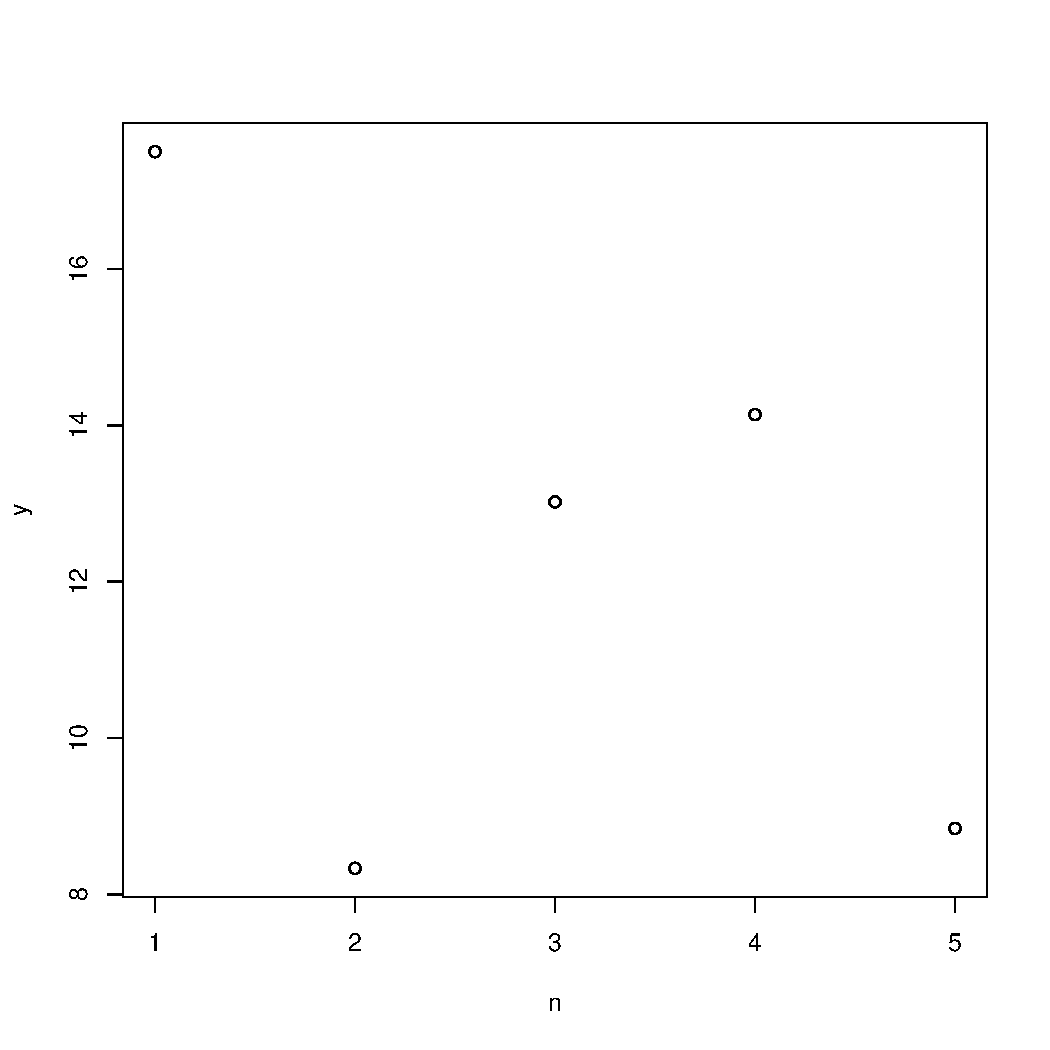
\includegraphics[width=\maxwidth]{figure/Chunk02-1} 
\end{knitrout}


\end{document}
